\chapitre{Aussi bien invoquer Quetzalcoatl, du vendredi 22 au dimanche 24 juillet 2033 }{Quand on n’a ni voiture pour se rendre au travail, }{ni Saguewanish pour circuler à l’interne, pourquoi devrait-on avoir accès aux services de télécoms ? N’est-il pas établi que les situations désagréables tendent toujours à proliférer, à s’organiser en bandes, à se concerter dans une surenchère éprouvante, à tout faire en leur pouvoir pour châtier lourdement, allez savoir pourquoi, la personne sur qui elles s’acharnent ? N’est-il pas documenté hors contestation que les objets inertes, les plus sournois étant ceux qu’on a gavés d’électronique, font généralement front commun pour nuire avec délectation aux humains, pour leur manifester toute la haine dont ils sont prodigues, pour tenter de les amener le plus douloureusement possible à leur perte ?  }

Surtout les êtres qu’ils détectent - ils en sont capables - comme étant accablés de problèmes intimes, familiaux et professionnels. On jurerait qu’ils disposent de capteurs évolués pour les repérer et les torturer encore plus cruellement. À preuve, quand Timothée a démarré une session musicale chez lui, tout à l’heure, son système lui a inopinément fait jouer un solo de trombone.

Ainsi, en arrivant au Centre, il constate que son dispositif personnel polyvalent (DPP), sa boucle d’oreille, ne fonctionne plus. Il l’a pourtant rechargé la veille, mais ce matin, le bidule semble avoir passé l’arme à gauche, probablement en ricanant. Qu’y a-t-il d’étonnant à cela ? Le gadget idiot ne fait que démontrer sa solidarité avec la franc-maçonnerie électronique encadrant la vie au XXIe siècle. Reste que Timothée a peine à refréner une violente pulsion l’incitant à aplatir le petit appareil à grands coups de talon.

De la cafétéria, Shimoune Saint-Pierre le salue de la main. Il a les yeux cernés, les traits terriblement tirés, mais il affiche un sourire qui en dit long sur l’aspect dissolu qui, de toute évidence, a caractérisé sa nuit. Timothée lui retourne un vague signe à peine esquissé et file directement jusqu’au 5e. En route, aucune rencontre détestable n’est à signaler et il ne croise pas Luce Morency. De plus, les gars du frigo n’ont pas l’air d’être en train de s’affairer sur son étage, les joueurs de 500 qui le voient passer ne l’affligent d’aucunes remarques et personne ne traîne au poste de garde. Dart Vader, lui, qui est dans la geôle du sous-sol, n’est pas là pour l’achaler avec ses histoires de nourriture. Quant à Jean Saint-Gelais, il ne semble pas rôder dans les couloirs; tant mieux. Par contre, arrivé au coqueron qui lui sert de bureau, il grimace devant l’impressionnante liste des appels à retourner : l’atelier mécanique, Robespierre, la secrétaire de Carl Michaud, le garage, Claude Sey et Marie-Odile Tremblay. Et sa boucle d’oreille est foutue. Qu’à cela ne tienne, il s’en remettra à son terminal. Moins pratique, absolument pas mobile, mais tout aussi efficace !

Le mécanicien lui apprend d’abord que sa Saguewanish a été sabotée, qu’il a fait un rapport et qu’il y aura enquête. Dès qu’il recevra le feu vert, il changera le bloc-moteur au complet; il a un «reconditionné» en stock. Mais en attendant, il ne peut pas lui prêter une bécane «de courtoisie», il n’en a plus depuis belle lurette. Désolé ! Faut se plaindre à la direction générale. Ensuite, Robespierre, le colosse au nez fourré partout, veut lui présenter quelqu’un, ou, plutôt, quelqu’une. C’est très important et le plus tôt sera le mieux. Une nouvelle histoire de Pétépano ? Quant à la secrétaire du DG, elle lui annonce la visite imminente de son patron ce matin même. Viendra-t-il avec des chiens mangeurs d’hommes, ou pire, avec Dauphin et ses Papyblues ? À son tour, le garagiste explique lui avoir changé ses pneus, mais une fois juché sur le monte-charge, le bazou a révélé que le réservoir à essence était pourri, qu’il coulait et qu’on devait le réparer d’urgence. Le problème était de dénicher la pièce de remplacement quelque part, ce qui, compte tenu de l’âge de la bagnole, n’était pas de la tarte. Il fallait prévoir plusieurs jours, peut-être même plus d’une semaine. Pour sa part, Claude Sey lui rappelle que le Flipper s’activait de plus en plus et qu’il avait désormais le docteur Gagnon dans son collimateur. De quoi tourner les talons et fuir dans le premier bar venu.

- Nous n’avons aucune trace numérisée des malfaiteurs, lui confirme Marie-Odile en fin de retour d’appels. Et puisque des pneumatiques, ça ne se crève pas par miracle et que l’homme invisible n’existe qu’au cinéma du siècle dernier, on a conclu que des gens avaient utilisé une carabine à gros plombs. Ça se vend dans les Wal-Mart. Ils ont dû s’arrêter sur la voie publique et, sans avoir peur de se faire filmer, ont tiré sur tes pneus. Va donc falloir que tu cesses de te stationner aussi près de la rue.

- Mais y pas d’autre place. Mon char est à essence …

- C’est vrai, désolée !

- De toute façon, je risque de ne plus avoir de char pour un bon bout de temps.

Il lui raconte son histoire de réservoir, puis déborde sur sa Saguewanish dont le bris criminel a probablement dû passer par le bureau de l’agente de sécurité. Elle lui demande s’il a des doutes sur le ou les coupables, ce à quoi il réplique par la négative, sauvant la mise du père Jean à qui, dans sa tête agitée, il entend régler le compte lui-même. Elle se dit intriguée par le fait qu’il est ainsi ciblé. Il lui répond que cet état de fait est probablement dû à sa personnalité marginale. Les gens voyagent en bancs de poissons, soutient-il, et si un individu semble suivre à côté du banc, certains, les éléments les plus méchants et, en même temps, les plus grégaires, en ressentent de l’agressivité et la manifestent. Parfois directement, mais la plupart du temps de façon hypocrite.

Marie-Odile sait de quoi il parle ! Elle le comprend parfaitement. N’est-elle pas elle-même «marginale» ?

- Je suis un peu forte des hanches, mon visage ne correspond pas aux canons de la beauté et en plus, je suis une agente de sécurité, une flic qui fait souvent des jobs de flic.

Pas besoin d’avoir de l’expérience ès bagatelle pour savoir que la Bitch ne semble plus vouloir agir comme son nom le laisse entendre. Même que, constate Timothée, elle vient de lui ouvrir une porte assez grande pour qu’en sorte et disparaisse tout l’Afrika Korps, cette légendaire armée du 3e Reich à laquelle appartient Hans le feldwebel SS, holotar botté et casqué présentement sur la glace. Elle lui a ouvert une porte assez grande pour qu’il y entre, lui le fils qui n’en peut plus, sans qu’il ne risque de se cogner l’ego ou de s’écorcher les sentiments. Si le ciel existe et s’il y a des saints, et si les saints ont déjà été des hommes, c’est maintenant qu’il faut qu’il y en ait un qui se manifeste pour aider l’inexpérimenté Timothée à saisir l’occasion au vol.

- Je pense que tu es injuste et dure avec toi. Mais moi, par contre, je n’ai rien pour moi.

Le «ben voyons» qu’elle lui répond constitue une sorte d’indication qu’elle pourrait ne pas le croire aussi moche qu’il semble vouloir le dire. Pour l’instant, il demeure en lice, mais la victoire n’est pas encore acquise. Il ne lui faut surtout pas en rester là; il manque au moins un point pour accéder à une partie gratuite. Timothée pour qui l’acte de séduction est une notion extravagante et inconnue, va devoir tenter la botte, la finale, celle de Jarnac. Bien entendu, son cœur s’est arrêté de battre et sa respiration ressemble à un moteur traditionnel dont l’alimentation en essence est infiltrée d’eau. Beaucoup plus tard, quand il se remémorera l’histoire, il comparera cet instant à celui vécu par un héros démineur qui, dans un film américain, à deux secondes d’une méga explosion qui aurait emporté quinze gratte-ciel, choisit de couper le fil vert alors que son camarade lui hurle de sectionner le rouge. Et ça marche !

\begin{floatingfigure}[l]{60mm}

\includegraphics[height=60mm]{corps/chapitre9/img/personnage-qz.jpg}
\end{floatingfigure}

- As-tu déjà goûté à la pizza mexicaine de Da Peperone ?

Après une courte hésitation, peut-être due à son étonnement, elle répond par la négative. Timothée qui se traite de con, poursuit, axphysié par l’angoisse, dans la même foulée, convaincu qu’il est en train de couler à pic au-dessus du Triangle des Bermudes.

- Je vais en manger une à midi… euh !

Silence à l’autre bout de la connexion.

- Une spécial Quetzalcoatl …

Mais quel sinistre con ! Et si elle lui rétorque qu’elle n’en a rien à foutre de ses petites habitudes du midi ? Ou si elle lui demande pourquoi il mange aussi mal ? Ou si elle lui dit qu’elle ne veut pas s’empoisonner avec ce quetzal coa machin ? Que va-t-il pouvoir répondre ?

- Une spécial quoi ?

- Euh … Quetzalcoatl. C’est un dieu, un serpent à plumes, chez les Mayas et les Aztèques, au Yucatan, au Mexique, euh … au Guatemala.

Que c’est mal engagé, que c’est mal engagé ! Pourtant, incrédule, il l’entend finir cette essentielle question qu’il n’a pas osé compléter.

- Tu me dis ça parce que tu souhaites que je t’accompagne ?

Elle lui a tendu une perche au plus profond de sa connerie.

- Oui.

Elle lui répond trouver la perspective intéressante et qu’elle voudrait bien y aller. Mais au même moment, on frappe à la porte de Timothée.

- Excuse-moi, j’ai quelqu’un … euh, on se retrouve là-bas ? Sur l’heure du lunch ?

- Je peux y être vers midi et quart.

- OK ! euh … merci ! À tantôt !

Carl Michaud vient d’entrer dans l’officine du chef de section. Il est seul comme un roi en goguette.

- Comment allez-vous, Monsieur Tardif ?

Timothée réalise qu’il n’a pas prévenu le père Asselin de cette visite du grand patron. Mais le vieillard étant assez ouvert, il ne devrait pas y avoir de difficultés, du moins l’espère-t-il. Et si le bonhomme en dit trop, s’il s’aliène le DG ? Si Michaud recherche seulement un prétexte grabataire pour saquer l’irrespectueux CS-1 ? D’un autre côté, cette visite peut chambouler la misérable vie du vieil informaticien. Par exemple, Michaud peut lui octroyer un droit à la résurrection et Asselin peut se retrouver pris en charge, soigné, redevenu utile.

- C’est par ici, monsieur. Suivez-moi, s’il vous plaît.

- Vous êtes à pied ?

- Ma Saguewanish a rendu l’âme. Le plus drôle, c’est que monsieur Asselin, l’ingénieur que nous allons visiter, m’avait prédit, au kilomètre près, le moment où ça arriverait.

Michaud fait comme si cela ne le concernait pas.

La salle 3P-M sent particulièrement mauvais ce matin et les deux visiteurs ont peine à contenir un réflexe de recul en entrant. Deux bénéficiaires alitées semblent agitées et une tend le bras vers le grabat d’Asselin. Comme le constate Timothée, il a ses écouteurs sur les oreilles, mais Tchekhov ne joue plus, le bidule s’est complètement déchargé. De toute façon, le bonhomme s’en fiche, il est mort.

- Et merde, s’exclame le chef de section.

Carl Michaud s’approche, regarde et sans demander son reste, sans un mot pour son employé, disparaît vers son étage climatisé où la senteur de la mort n’est qu’une théorie sur papier.

Consterné, Timothée lorgne le vieil ingénieur et lui enlève le petit casque d’écoute. Puis, il lui replace délicatement les cheveux, tente de lui joindre les mains, ce qui s’avère impossible, et lui remonte le drap jusqu’au menton. Après un moment de recueillement, il quitte la pièce le cœur gros. Privé de sa boucle d’oreille, il doit se rendre au poste de garde pour enclencher la procédure nécessaire. Or, c’est sur Bérubé qu’il tombe.

- Michel Asselin est mort cette nuit. Peux-tu aller commencer ce qu’il faut faire pendant que j’avise le frigo et l’hébergement ?

- J’ai pas ben l’temps, Motté, faut que j’m’occupe des trois bénévoles qu’on nous envoie à matin !

- Laurent, je t’ai pas dit de t’occuper des bénévoles, mais d’aller vider le tiroir de monsieur Asselin, de ramasser ses affaires, incluant ses papiers et m’amener tout ça ici. As-tu compris, câlisse ?

Le préposé qui note le «câlisse» identique à celui de la veille, juge à propos d’obéir et il file vers la salle 3P-M. Dans son bureau, Timothée avertit d’abord «les gars du sac noir» puis il appelle chez Lemoignan, le salaud responsable de l’hébergement. C’est l’adjointe administrative qui répond et qui s’étonne quand elle entend l’objet de l’appel.

- Ça fonctionne l’informatique à matin, tu peux faire ton rapport directo. En passant, occupe-toi donc de tes deux autres morts, pour une fois que ça marche !

- Écoute, j’ai pas grand temps et, surtout, j’ai pas le cœur à ça !

- Là, mon beau Motté, c’est ton problème ! Veux-tu que Jean-Pascal te rappelle ?

- Non.

- Il avait de la famille ?

- Des sans-cœur qui l’ont dépossédé.

- Faut quand même que je les avise. Méchant début de journée. J’ai une moyenne de deux morts par étage à matin. On dirait qu’ils se sont tous donné le mot pour péter au frette.

Le CS-1 raccroche. Le système informatique fonctionne comme s’il s’agissait d’un symbole imaginé en l’honneur de Michel Asselin, 1951 – 2033, informaticien-choc décédé pour cause de privations existentielles.

- Maudite époque de marde, fait-il à son terminal.

Comme Bérubé est revenu avec les quelques possessions du vieillard, Timothée les lui fait enfouir dans le grand sac réglementaire, incluant le petit gadget audio. Puis, sans rien attendre de son subalterne, il s’en retourne vers la dépouille se recueillir au pied du lit dans l’attente des employés de la morgue.

- T’as une minute ?

C’est Robespierre qui vient d’entrer dans la salle. Apercevant le cadavre, il s’approche doucement.

- Ton monsieur d’informatique ?

- Oui.

- Dommage. Je peux te parler ?

- Non.

- Pas grave. Je vais t’accrocher plus tard.

Le corps parti, Bérubé revient pour s’occuper du lit et Timothée regagne son bureau où patientent les trois bénévoles. Il a tôt fait de leur distribuer des tâches et va prendre place devant son terminal. Pas pour travailler, pour ruminer son sort, pour faire le point, pour réfléchir sur le fait que son domicile est devenu une souricière où de gros minets sont à la veille de lui payer une visite qu’il ne pourra empêcher, que son travail est désormais un cauchemar plein de monstres dont l’inhumanité est proportionnelle à leur rang dans la hiérarchie, que sa vie personnelle est plus pitoyable de jour en jour, que ses chances d’être heureux sont nulles, que ses ressources financières se sont volatilisées et que son espérance en une certaine qualité de vie n’est plus. Pire, il doit tout à l’heure aller faire le beau, tâche dont il ne connaît ni l’alpha, ni l’oméga, devant quelqu’un qui pourrait, quelque part, éventuellement, dixit Shimoune Saint-Pierre, être un début de clé vers la grande console à lumières dont son existence aurait un immense besoin. Pour parler en euphémisme ! Pour réagir à cette panoplie épouvantable d’ennuis et de désagréments assortis, il n’a d’autre choix que de se dresser. Il est tenu de tout affronter en héros résigné ! Debout sur la proue, près de l’étrave, face au crachin de l’Atlantique Nord. «Je t’aurai Moby Dick !» Sa mère n’a plus que lui pour survivre. Même chose, sûrement, pour son père. Si le fils binoclard, pansu, chauvasse, puceau et équipé d’un prénom que ridiculise sa nature de nono, de raté qui ne pourra jamais rajouter de cordes à un outil d’expression qui le fera passer à l’histoire, bref si ce concentré de mocheté laisse tomber, ils mourront. Pour le moins ! Voilà quand même un incitatif de taille pour qu’il cesse de s’apitoyer sur son petit sort tata, non ?

C’est dans cet état de lucidité qu’il entreprend la préparation de ses rapports de décès. Trois morts, trois places libérées, trois nouveaux occupants, trois nouveaux fichiers, trois nouveaux jeux de peines, d’angoisse, de détresse.

- Chef, j’ai un bout de papier pour toi !

Timothée se retourne et aperçoit le visage pétant de santé de Solange Gadoury. Un instant, il songe à lui interdire l’accès à son bureau. Mais il n’en a pas le temps. La grassouillette matrone est déjà à côté de lui.

- Tape ce code quand ça t’adonnera et les 642 piastres d’avant-hier du père Lafrance vont entrer dans ton compte !

- Ça n’a pas de bon sens, madame Gadoury. Votre protégé est très malade. Il emplit ses couches aux heures. Au moins, aux heures ! J’ai personne qui veut s’en occuper. Son cas est rendu trop lourd.

- 642 belles piastres, chef !

Que dirait la Maririou ? Sûrement quelque chose comme «arrête de niaiser et fais ce qu’il faut pour ramasser ce bel argent; on en a besoin !»

- Attendez-moi ici, madame Gadoury, j’ai peut-être une idée.

Un coup d’œil à sa montre et il file vers le salon communautaire où vivote la faune habituelle.

- Monsieur Jean, j’ai affaire à vous, dit-il au bonhomme qui vient d’annoncer huit cœurs.

- J’suis pas mal occupé, mon Motté.

- Dans ce cas-là, j’vais vous parler devant tout le monde.

- OK, mais fais ça vite.

Timothée qui s’est approché de la table, entreprend d’enferrer le vieux malfrat de cette voix douce, calme, presque basse, qui le caractérise.

- Le moteur de ma bécane a sauté et la réparation va coûter au-dessus de 2 500 \$.

- Que c’est que tu veux que ça me fasse ?

- Étant donné qu’elle a été habilement sabotée, ils ont décidé de faire une enquête. Et ils vont finir par savoir que vous êtes technicien Saguewanish certifié. En plus, il y a sûrement quelques-uns de vos amis qui vont leur bavasser que c’est vous le coupable. S’ils me l’ont colporté à moi, vos bons amis, ils vont probablement en faire autant avec les flics. Autrement dit, vous êtes dans la grosse misère. Le vandalisme sur le bien public est un acte hautement répréhensible prévu dans le Code criminel. N’importe quel juge va vous condamner.

La perfidie vient de se trouver une nouvelle icône. Plus personne ne parle, ni ne fait de bruit.

- T’es malade, le Motté, finit par rétorquer le bonhomme. Tu m’accuses sans preuve. C’est qui qui t’a dit que c’était moi ? Hein ? Nomme-le ‘sti !

- On se reparlera de ma maladie, de mes preuves et de mes sources dans quelques jours quand ils vous auront coincé et descendu finir vos jours au sous-sol. Mais, d’un autre côté …

Timothée hésite et ne semble pas vouloir continuer sa phrase. Au fond de la pièce, madame Bellow sourit dans son livre.

- De quoi ?

- Ben je peux m’arranger pour qu’ils vous foutent la paix, ment-il. Il vous suffirait d’être gentil.

- Que c’est que tu veux dire ?

- Pas grand-chose. Juste de vous occuper du père Lafrance. Il en a plus pour longtemps.

- M’en occuper ?

- Oui, à chaque jour à partir de 16 heures pour le reste de la semaine, je n‘ai plus de bénévoles. Vous lui tenez compagnie jusqu’à ce qu’il soit bien parti pour sa nuit, vers 21 heures. Entre autres, ça veut dire de lui changer ses couches à toutes les heures. Si la police vient pour vous ramasser, je pourrai leur expliquer que je ne peux me passer de votre dévouement, que je n’ai personne pour vous remplacer, que vous êtes la gentillesse même, que vous êtes un intervenant bénévole exemplaire et que, dans le fond, ma Saguewanish, vous l’avez bricolée pas pour commettre un crime, mais pour me taquiner puisqu’on est de bons copains.

- Y en est pas question !

- OK. Une fois au sous-sol, vous saluerez Dart Vader de ma part !

Et le Timothée de quitter le salon. Jean met cinq courtes secondes pour réagir.

- Eh, minute ! On peut en discuter, non ?

- Y rien à discuter, monsieur Jean. Vous aidez votre ami Lafrance, ou vous ne l’aidez pas. C’est tout.

- Astie de chien sale ! Je commence quand ?

- Aujourd’hui. Suivez-moi.

Au poste de garde, ce Timothée «nouveau genre» présente la situation à Mérovée et lui demande de préparer «ce bénévole inspiré» qui entre en fonction l’après-midi même. Heureusement que les verres du vieillard sont aussi épais, sinon l’intensité de la haine que le CS-1 y discerne le fustigerait sur place.

Et c’est presque en souriant qu’il s’en retourne à son bureau expliquer le rebondissement à Solange Gadoury. Alors, la conscience tranquille, il accepte le petit papier. Et puis pourquoi ne l’aurait-il pas fait ? 642 \$ quand on est moribond et sans succession, ce n’est rien. Mais 642 \$ quand on nage dans les ennuis, ça permet de se garder le nez hors de la vase deux ou trois jours de plus.

Peu après, Timothée est chez Da Peperone, assis sur le bout des fesses en face de Marie-Odile. Comme c’est la coutume sur l’heure du midi, l’établissement a fait le plein avec des cols bleus, la voirie municipale occupant un grand terrain deux rues plus au sud, avec des travailleurs du complexe commercial qui s’étire de l’autre côté de la chaussée, avec du personnel du Centre régional pour les personnes handicapées intellectuelles, le C2R2HI, dont on aperçoit la sinistre construction de la fenêtre du resto et, malheureusement pour l’agente de sécurité et le chef de section, par des employés du CRG-BSL dont l’édifice est à deux pas. C’est ce qui explique que leur inoffensif rendez-vous, repris sous forme de médisance croustillante, déferle partout au Centre à la vitesse de l’éclair. Tellement que même Shimoune absorbé dans sa distribution de manger mou, en apprend une variante : «Apparemment, la Bitch se fait sauter par le Motté».

Autour d’une «médium Spécial Quetzalcoatl» avec «extra piments forts», on parle d’abord des déboires de Timothée, de certains déboires s’entend, soit de sa boucle d’oreille qu’il devra remplacer, de sa voiture qui est en réparation et de sa Saguewanish qu’on soupçonne d’avoir été sabotée. Telle que présentée, l’histoire arrive même à dérider Marie-Odile. Évidemment, Timothée se garde bien de mentionner le père Jean. Peut-il faire confiance à cette femme flic ? En fait, il parle très peu. Puisqu’il craint de passer pour idiot, puisqu’il est gêné et empêtré dans son langage corporel empoté, il ne fait qu’exacerber son absence naturelle d’éloquence. Heureusement, Marie-Odile compense. Elle a la jactance nerveuse. Elle papote. Elle jacasse pour combler le vide. Elle dérape même sur les mièvreries. Et la voilà qui livre quelques pages bien senties sur son boulot, ce qui n’a rien d’étonnant, les gens étant ainsi faits. Puis, au terme d’une rapide transition qui recalerait un étudiant au bac, elle déborde sur sa vie personnelle, une vie ennuyante, semble-t-il, où rien n’arrive jamais. Pas de sorties théâtre ou ciné, jamais de soirées au restaurant, il y a au moins dix ans qu’elle n’a pas voyagé et elle ne pratique plus de sport. Ça commence à paraître et elle est à la veille de faire quelque chose. Mais elle ne sait trop par quel bout prendre cela. Ses seuls loisirs sont le ciné-maison et Internet. Pas un mot sur Ilsa la louve des SS.

Et pour cause, elle s’occupe de ses parents qu’elle visite presque tous les jours, deux braves vieillards encore aptes à se débrouiller qui viennent d’atteindre 79 ans et qui sont sans le sou. Ils ne gagnent plus suffisamment pour vivre de façon autonome et Marie-Odile doit leur consacrer une partie de ses revenus. C’est son père le pire, explique-t-elle. En raison de l’usure générale de son corps, il ne peut plus exercer son métier de serveur. L’arthrite et les maux de dos ont fait leur œuvre. De plus, c’est un vieux noceur qu’elle-même se trouve incapable de gérer; le bonhomme est imprévisible, un «loose cannon » comme disent les Montréalais. Quant à leur bungalow, il date de 1967 et est en très mauvaise condition. Le pire c’est qu’il est hypothéqué jusqu’au trognon. Bref, elle craint pour eux s’ils se retrouvent «placés» au CRG-BSL. La loi du Gros Turcotte est implacable : dès qu’on coûte plus cher qu’on rapporte, on est «pris en charge». Il faut travailler dans une telle institution pour avoir, n’est-ce pas, une très bonne idée de ce qui pourrait trop rapidement leur arriver. Mais, bon, a-t-on le choix ? Tout cela l’angoisse terriblement.

Dès lors, tous les ingrédients sont en place pour que survienne la question tant redoutée.

- Et toi, ton père, ta mère ?

Ce qu’il ressent alors pourrait être classé comme étant un arrêt cardio-respiratoire. Sauf qu’il est conscient de l’énorme bêtise qu’il a commise en s’imaginant pouvoir amadouer et manipuler cette femme qu’on lui a présentée comme étant la «clé» de sa survie. Il est hors de question qu’elle apprenne comment il s’occupe, lui, de ses parents. Elle est flic. Elle va le traîner à coup sûr jusqu’à la guillotine ou la chaise électrique la plus près du CRG. Puis, devant une populace haineuse, lanceuse de tomates avariées, de crottin mou et de cailloux, elle se fera aller le bras séculier. Ce sera Schlac!, ou Zap!, selon le cas. Timothée sait une chose : même si son silence s’inscrit dans son comportement général, celui adopté en début du Spécial Quetzalcoatl extra piments forts, il lui faut réagir. Impérativement réagir. Il doit triompher de ce redoutable écueil. Le reste de sa vie en dépend. Mais en même temps, il ne peut répondre à une telle question. Comment le pourrait-il ? Sauf que s’il ne dit rien de valable, tout est foutu ! Il n’a d’autre choix que de redémarrer la machine. Sans erreur possible !

Ainsi, il la regarde et se lance dans le vide.

- C’est moi le joueur derrière cet holotar qui se prend pour Roméo et qui s’est amouraché d’une Juliette esthétiquement remaniée, un holotar que je soupçonne d’être à toi.

Elle le fixe d’abord sans expression, comme si ses yeux étaient devenus deux scanneurs de haute précision. Puis, quelques instants plus tard, elle les illumine d’un sourire qui pourrait la faire passer pour belle.

- Je m’en doutais bien.

L’étape suivante est cruciale. Les représentants commerciaux l’appellent «closing» et les Français, «emballage de la nana». Il s’agit maintenant de consolider les acquis, de les transformer en quelque chose de définitif, de momentanément ou de temporairement définitif. Que dire ? S’essayer avec un poncif hollywoodien comme «on va chez toi ou tu viens chez moi, bébé ?» Timothée est complètement démuni. Démuni comme un coq à viande miraculeusement échappé d’une des mille cages d’un camion en route pour l’abattoir et qui se retrouve dans un poulailler plein de grosses poules lourdement expérimentées. Il faut se rappeler que c’est la première fois de sa vie que le fils de la Maririou travaille une femme au corps.

C’est Marie-Odile que l’on ne dirait guère mieux outillée, qui attaque pourtant, toute chattemite.

- Penses-tu qu’on va continuer à jouer à Roméo et Juliette avec nos holotars ?
Il fixe le reste de pizza tellement la question est insupportable. Quetzalcoatl, dieu de Da Peperone et des Mayas, serpent à plumes à qui on doit la perte de Moctezuma, fais quelque chose, sacrament ! Aide-moi à me tirer de ce merdier !

- Ben, euh …

- Ben, j’sais pas, moi, à c’t heure qu’on se connaît ….

- Euh … c’est vrai qu’on pourrait se passer de machines pour un bout de temps …

- Ouin !

Un silence gênant vient les éprouver. C’est la serveuse qui casse la glace en s’informant s’ils ont aimé la pizza. Tous deux opinent du chef en se zieutant du coin de l’œil. Dans sa tête, Timothée entend une sorte de mantra l’amener tranquillement vers la folie: «faut closer», «faut closer», «faut closer» ! Il revoit ce lieutenant parachutiste crier «Go go !» à ses GI qui se précipitent un à un en dehors de l’avion. Il fonce.

- Euh, ça te tenterait-tu qu’on remette ça ?

Encore une fois, ses yeux viennent s’illuminer et elle redevient belle.

- Ouin, ça serait le fun, quand ?

Quetzalcoatl, à l’aide ! Je me meurs !

- Euh … je sais pas, ce soir ?

Elle sourit davantage. Timothée est encouragé. Ça marche, sacrament !

- Euh … on pourrait aller Au Vieux Cormier, ils ont du pas pire manger et ils sont pas chers …

- C’est vrai, j’aime ça c’t endroit-là, ment-elle.

Toc-schloc toc-schloc toc-schloc, fait son pauvre cœur.

- À quelle heure ?

- B’en j’sais pas, euh, 19 heures ?

- OK, j’vas être là !

Pas croyable ! C’est gagné. Jamais il n’a été aussi fier de lui, le Timothée-Milet, une femme vient de lui dire oui ! À lui ! Il a fait ce qu’il devait et ça a marché. Mais il ne s’agit pas de n’importe quelle femme. C’est la Tremblay, une flic, la clé potentielle d’un début de solution.

Méprisant les petits regards mesquins, les éclats furtifs de rire hypocrites, tous deux réintègrent leurs locaux au CRG, elle au 2e, lui au 5e. Si avant de prendre l’ascenseur il a dû saluer l’inquiétant docteur Bellavance qui l’a gratifié d’un «comment allez-vous, monsieur Tardif», en le quittant, il aperçoit Mme Thériault et Mme Labbé entrer furtivement dans le salon communautaire. L’idylle semble durer, pense-t-il. Mais il a bien d’autres soucis en tête et ces deux vilaines mémères ne font pas le poids : ce soir il lui faut absolument en arriver au sens ultime de l’expression «devenir un homme». Cela, sans Petepano, se dit-il, en voyant Robespierre lui faire signe.

- J’ai quelqu’un à te présenter, lui répète le désœuvré permanent. Une madame Martin qui veut te parler sans faute.

- C’est qui ?

- Une infirmière, quelqu’un dans mon cercle d’amis.

- Elle me veut quoi ?

- Pas de mes oignons. Mais je la connais assez pour savoir que c’est sérieux.
Béatrice Martin était une idéaliste dans la jeune quarantaine qui, pendant une quinzaine d’années, avait tenu un dispensaire en Haïti. Depuis six mois, elle était de retour à Rimouski, malade et épuisée, et, par un hasard de circonstance, avait fraternisé platoniquement avec Robespierre, «le plus grand cœur de ce côté-ci du fleuve». Or, hier soir, dans le cadre d’un mini cocktail entre copains, elle avait posé des questions sur Timothée, un Tardif qui pourrait être le fils de Marie Rioux, la fille d’une amie très chère de sa grand-mère. Puisque cette Rioux avait naguère épousé un certain Romain Tardif et qu’ils avaient eu un garçon appelé Timothée, un nom quand même rare, elle se demandait si ce compagnon de travail de Robespierre pouvait, par le plus grand des hasards, être apparenté à cette Marie. Si cela était possible, elle avait un document de première importance à lui remettre.

- Elle a su comment que toi et moi étions collègues ?

- Je racontais comment le personnel du CRG était baveux, méchant, désagréable, arrogant, bref, chiant auprès des vieux. Alors, j’ai parlé de toi comme étant un cas unique faisant tout le contraire. Et c’est en nommant ton nom qu’elle a réagi. Elle nous attend dimanche après-midi chez elle. Je passe te prendre ?

- J’ai plus de char !

Robespierre tourne les talons.

- Fais attention à toi, mon ami.

Quelques heures plus tard, Au Vieux Cormier, tout va se dérouler comme dans un film à l’eau de rose, comme dans un roman où le pathos se transvase au kilo, comme dans un soap californien où l’héroïne siliconée sur le retour fait semblant de ne pas trouver cucul la passe de son Casanova de banlieue, bref, comme dans une vie imaginée par ceux qui n’en ont pas. Les dialogues seront lamentables, les premiers sourires tendus et les manières de table ampoulées. Quant aux épanchements, ils nécessiteront une bouteille de pinot noir estrien avant de pouvoir démarrer. Mais dès ce moment, ce sera une course à la «qui perd gagne» entre ces deux êtres privés de rapports humains, pour savoir lequel des deux confiera le plus de secrets à l’autre.

Et lorsque, vers les 22 heures, ils finirent par convenir d’aller chez elle, ce fut dans un contexte épouvantable de malaise, de gêne aussi paralysante qu’une morsure de serpent mexicain - «Quetzalcoatl, aide-moi, sacrament !» - de souffrance déclencheur d’infarctus, de peur, de désir, d’angoisse et d’appétit tout entremêlés. Puis, il fallut tenir inutilement des propos vides pendant une grosse heure avant d’accéder, toc-schloc toc-schloc toc-schloc, au tabernacle du sanctuaire. Et là il fallut encore un solide quinze minutes avant que Marie-Odile n’ait le courage d’enlever l’éclairage. «Te Deum laudamus» ! En passant sous silence l’impressionnante collection de maladresses commises de part et d’autre, on peut dire que quand, aux petites heures, Timothée appela un taxi avec la boucle d’oreille de Marie-Odile, l’inévitable avait été consommé. À 43 ans, « jouez hautbois, résonnez musettes », le fils de la Maririou avait perdu son pucelage, grâce au patient vouloir d’une agente de sécurité chattemite en mal hurlant d’affection, «Chantons tous son avènement !».

Sauf qu’il le lui avait avoué. Inutilement avoué doit-on croire, puisqu’elle s’en était aperçu dès la première minute. Non pas qu’elle était une rombière expérimentée, mais, au fil de sa vie d’adulte mal lunée, elle avait acquis un peu d’expérience, le mot «peu» se référant ici à un calcul pouvant être établi sur les doigts d’une seule main.

C’était donc ça, faire l’amour, sentir un corps féminin sur soi, vibrer avec quelqu’un dans une intimité exultante, oublier, un instant, qu’on était un binoclard grassouillet à moitié chauve de qui la planète entière se moquait. Plonger, tête première, dans les entrailles chaudes, humides, sans fonds, insatiables d’une cousine, si ce n’est la petite sœur par la fesse gauche, du redoutable Quetzalcoatl, question d’y fouiner en toute liberté, les truffes du juste bonheur.

C’est ce qui explique que le lendemain, au début de l’après-midi, après s’être assuré que tout se passait normalement – un bien grand mot – chez ses parents, Timothée va, pour la première fois de sa vie, connaître la sensation de se présenter chez une dame «la bitte sous le bras». Cette fois il ne faudra que cinq minutes avant que l’on troque son babil idiot contre une session d’effusions, d’abandon et de rattrapage par rapport à leur vie cruelle.

Pourquoi fallut-il, Dieu du ciel, que ça prenne 43 ans ?

\begin{floatingfigure}[l]{40mm}
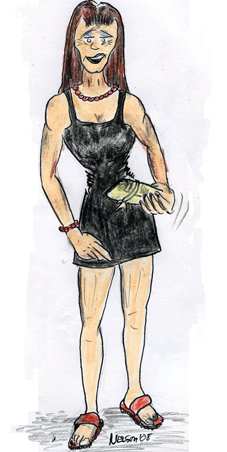
\includegraphics[height=60mm]{corps/chapitre9/img/personnage-beatrice.jpg}
\end{floatingfigure}

Béatrice Martin était une femme plus mince que menue, plus belle et attirante que sexy, que de coquines pattes d’oie avaient commencé à décorer, on aurait dit, pour le mieux. Sûre d’elle dans sa petite robe noire, elle les avait accueillis, Timothée et Robespierre, avec beaucoup de chaleur et leur avait offert de la bière. Puis, elle était rapidement passée au vif du sujet, une histoire, somme toute assez triste relative à sa grand-mère Joncas, Rose de son prénom, qui avait travaillé une bonne partie de sa vie dans un magasin de coupons de Rimouski. Or elle s’y était liée d’une grande amitié, semble-t-il, avec une nouvelle employée, Marceline Rioux, une malheureuse très amochée par la vie, qui mourut quatre ans plus tard en 1968. Sentant sa fin proche, la pauvre dame avait confié une forte enveloppe à Rose, lui faisant promettre de la remettre à sa fille advenant qu’elle décède. Mais quand cela se produisit, il ne fut pas possible d’accomplir cette ultime volonté. Retrouvée à Québec, la jeune femme refusa aussi bien le manuscrit que le signet mortuaire imprimé à la mémoire de Marceline. La bonne Rose dut redescendre, bredouille, à Rimouski. Peut-être par sentiment de culpabilité, elle conserva le document toute sa vie et, à la fin de ses jours, la laissa à sa fille, Jacinthe Martin, à qui elle raconta toute l’histoire.

- C’était ma mère. Et, je sais pas trop pourquoi, elle a choisi de ne pas s’en débarrasser. Elle l’a placée au travers de ses papiers importants, ses polices d’assurance, ses placements, etc. Quand elle est morte, le printemps dernier, j’ai commencé à faire le ménage dans sa paperasse. Dieu sait qu’il y en avait, ma mère était une ramasseuse. Mais, quelque part, ça tombait bien, j’étais en convalescence. C’est ainsi que j’ai découvert l’enveloppe. Intriguée, je l’ai ouverte et j’y ai trouvé une très longue lettre, un récit très touchant que j’ai lu sans pouvoir m’arrêter. J’en suis désolée. Mais, ç’a été un mal pour un bien, car la gravité du contenu m’a incité à vous retrouver, monsieur Tardif.

- Euh … merci madame.

- Vous êtes bien le fils de Marie Rioux dont le mari était Romain Tardif ? Des gens de Saint-Anaclet qui ont péri, me semble, aux alentours de 2027.

Que répondre ? Que ses parents ne sont pas morts, mais vivent présentement un enfer à l’autre bout de la ville, dans Nazareth ? Que lui, il est en train de devenir dingue avec cette histoire ? Qu’il se farcit une femme flic pour avoir une chance de voler des produits pharmaceutiques qui pourront acquitter une dette contractée auprès du shylock d’Esculape.

- Oui, répond-il, tandis que Robespierre corrobore de plusieurs signes de tête.
Elle lui tend une enveloppe un peu salie et jaunie, une enveloppe format lettre tellement bourrée qu’il a fallu la ficeler pour qu’elle tienne fermée.

- Alors, j’imagine que le contenu va vous prendre aux tripes.

Lentement, comme s’il présidait une cérémonie religieuse, Timothée retire la ficelle et ouvre le petit paquet. Il en extirpe une liasse de feuilles manuscrites. Sur le dessus, une page pliée en trois attire son attention. Elle est datée du lundi 27 mars 1967. Le texte est court et inquiétant :

- «Il est arriver un dramme dans la vie de Marie ma fille de 16 an et depuis ce temps la elle m’a fuit et a les devenu renfermé et tout le tant triste. Elle était déjà pas du monde mais ces devenu pire. Elle croix que cet pas à cause d’elle que j ai tuer son pére que cet juste à cause de moi que je lé pas défendu que j me suis juste vanger. SVP, quand je serai morte, remetter lui cette lettre. Je conte toute l’histoire. Merci.»

- Mon Dieu !

Timothée replace maladroitement les feuillets dans l’enveloppe.

- Euh, madame Martin, faut que j’aille lire ça à tête reposée.

- Je comprends.

- Euh … je sais pas trop comment faire pour vous remercier.

- Venez prendre un verre avec Robie (Robie ?, tiens tiens) de temps à autre. Ça va me faire plaisir.

Sans tenir compte de Gazou qui, encore une fois, veut le dévorer, Timothée s’approche de son père en train de regarder sa télé sans son, tandis que sa conjointe dort. Il lui tend la feuille pliée en trois.

- Faut que tu lises ça.

- C’est quoi ?

- Lis.

Quelques instants plus tard, les deux hommes se regardent.

- Veux-tu ben me dire c’est quoi c’t’affaire-là ?

- Faudrait lire toute la liasse pour le savoir.

Le bonhomme se lève, ce qui fait gronder le chien-rat.

- Mon Dieu Seigneur ! J’aime pas ça, c’t histoire-là. Viens, on monte chez toi, tu vas me faire la lecture, Timothée-Leary. Ici, on va déranger ta mère. J’ai de la misère avec mes yeux et c’est écrit plein de fautes avec des pattes de mouche. Mais avant, je pense que je vais mettre mon pied au cul de ce p’tit calvaire de chien lette !

Ce qu’il ne fait pas, bien entendu.

Arrivés à l’étage, ils s’installent dans le salon où, en moins d’une heure, ils vont voir défiler une histoire épouvantable, celle d’une petite victime qui, devenue adulte, continuera inutilement de l’être. Jusqu’à aujourd’hui.

- Lis mon Timothée !